\begin{frame}
  \frametitle{¿Qué es un Sistema Operativo?}
  \begin{itemize}
	  \item Es parte esencial de cualquier sistema de cómputo
	  \item Es un programa que actúa, en principio, como intermediario entre el usuario y el hardware
	  \item Su propósito: crear un entorno cómodo y eficiente para la ejecución de programas
	  \item Su obligación: garantizar el correcto funcionamiento del sistema
	  \item Sus funciones principales
		  \begin{itemize}
			  \item Administrar la memorio
			  \item Administrar la CPU
			  \item Administrar los dispositivos
		  \end{itemize}
  \end{itemize}
\end{frame}

\begin{frame}{¿Qué es un Sistema Operativo? (cont.)}
  \begin{itemize}
  \item Según Wikipedia:
  
   \textit{``...Es un conjunto de programas de computación destinados a realizar muchas tareas...''}
  \item Según un usuario stándar: ``Lo que aparece cuando prendo la PC''
  \item ...
  \end{itemize}
\end{frame}

\begin{frame}
	\frametitle{GNU/Linux}
	\begin{itemize}
		\item Es un Sistema Operativo tipo \textit{Unix} (Unix like), pero libre
		\item S.O. diseñado por miles de programadores
		\item S.O. gratuito y de libre distribución (se baja desde la Web, CD, etc.)
		\item Existen diversas distribuciones (customizaciones)
		\item \alert{Es código abierto}, lo que nos permite estudiarlo, personalizarlo, auditarlo, aprovecharnos de la documentación, etc...
	\end{itemize}
	\centerline{\alert{Podemos ver como está hecho!!!}}
\end{frame}

\begin{frame}
	\frametitle{¿GNU?}
	\begin{itemize}
		\item GNU = \textbf{G}NU \textbf{N}o es \textbf{U}nix
		\begin{figure}
			\centering
			
\includegraphics[scale=0.2]{images/gnu.png}
		\end{figure}
		\item Iniciado por \emph{Richard Stallman} en 1983 con el fin de crear un Unix libre (el sistema GNU)
		\item Para asegurar que el mismo fuera libre, se necesitó crear un marco regulatorio conocido como GPL (General Public License de GNU)
		\item En 1985, Stallman crea la FSF (Free Software Foundation), con el fin de financiar el proyecto GNU
		\item En 1990, GNU ya contaba con un editor de textos (Emacs), un compilador (GCC) y gran cantidad de bibliotecas que componen un Unix típico.
		\item Faltaba el componente principal $\rightarrow$ El Núcleo (\textit{Kernel})
	\end{itemize}
\end{frame}

\begin{frame}
	\frametitle{GNU}
	\begin{itemize}
		\item Si bien ya se venía trabajando en un núcleo conocido como \textit{TRIX}, es en 1988 que se decide abandonarlo debido a su complejidad (corría en hardware muy costoso)
		\item En este momento se decide adoptar como base el núcleo \textit{MACH} para crear \textit{GNU Hurd}, el cual tampoco prosperó
		\item \emph{Linus Torvalds} ya venía trabajando desde 1991 en un Kernel denominado \textit{Linux}, el cual se distribuiría bajo licencia GPL
		\item En el año 1992, Torvalds y Stallman deciden fusionar ambos proyectos, y es allí donde nace \textit{GNU/Linux}
		\item GNU/Linux pertenece al desarrollo del software libre	
	\end{itemize}
\end{frame}

\begin{frame}
	\frametitle{GNU (cont.)}
	\begin{itemize}
		\item GNU se refiere a 4 libertades principales de los usuarios del software:
		\begin{itemize}
			\item Libertad de usar el programa con cualquier propósito
			\item Libertad de estudiar su funcionamiento
			\item Libertad para distribuir sus copias
			\item Libertad para mejorar los programas
		\end{itemize}
		\center{\textit{``Los programas son una forma de expresión de ideas. Son propiedad de la humanidad y deben ser compartidos con todo el mundo''}}
	\end{itemize}
\end{frame}

\begin{frame}
	\frametitle{¿Software libre?}
	\begin{figure}
		\centering
		\fbox{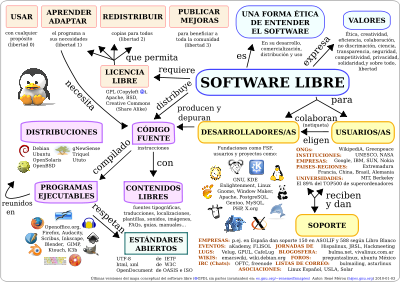
\includegraphics[scale=0.6]{images/freeSoft.png}}
	\end{figure}
\end{frame}

\begin{frame}
	\frametitle{¿Software libre?}
	\begin{itemize}
		\item Características del software libre:
		\begin{itemize}
			\item Una vez obtenido, puede ser usado, copiado, estudiado, modificado y redistribuido libremente
			\item Generalmente es de costo nulo $\leftarrow$ Es un gran error asociar el software libre con el software gratuito $\leftarrow$ Pensar en software gratis que se distribuye con restricciones
			\item Es común que se distribuya junto con su código fuente
			\item Corrección más rápida ante fallas
			\item Características que se refieren a la libertad de los usuarios para ejecutar, copiar, distribuir, estudiar, cambiar y mejorar el software
		\end{itemize}
	\end{itemize}
\end{frame}

\begin{frame}
	\frametitle{¿Software propietario?}
	\begin{itemize}
		\item Características del software propietario:
		\begin{itemize}
			\item Generalmente tiene un costo asociado
			\item No se lo puede distribuir libremente
			\item Generalmente no permite su modificación
			\item Normalmente no se distribuye junto con su código fuente
			\item La corrección de fallas esta a cargo del propietario
			\item Menos necesidad de técnicos especializados
		\end{itemize}
	\end{itemize}
\end{frame}

\begin{frame}
	\frametitle{GPL: Generic Public License}
	\begin{itemize}
		\item Licencia Pública General de GNU
		\item Creada en el año 1989 por la FSF
		\item Su objetivo principal es proteger la libre distribución, modificación y uso del software GNU
		\item Su propósito es declarar que todo software publicado bajo esta licencia, es libre y esta protegido teniendo en cuenta las 4 libertades principales ya vistas
		\item La versión actual de la licencia es la 3
	\end{itemize}
\end{frame}

\begin{frame}
	\frametitle{Características generales de GNU/Linux}
	\begin{itemize}
		\item Es multiusuario
		\item Es multitarea y multiprocesador
		\item Es altamente portable
		\item Posee diversos intérpretes de comandos, de los cuales algunos son programables
		\item Permite el manejo de usuarios y permisos
		\item Todo es un archivo (hasta los dispositivos y directorios)
		\item Cada directorio puede estar en una partición diferente (/temp, /home, etc.)		
		\item Es case sensitive
		\item Es código abierto
	\end{itemize}
\end{frame}

\begin{frame}
	\frametitle{Diseño}
	\begin{itemize}
		\item Fue desarrollado buscando la portabilidad de los fuentes
		\item Desarrollo en capas
		\begin{itemize}
			\item Separación de funciones
			\item Cada capa actúa como una caja negra hacia las otras
			\item Posibilita el desarrollo distribuido
		\end{itemize}
		\item Soporte para diversos File Systems
		\item Memoria virtual = RAM + \textit{SWAP}
		\item Desarrollo mayoritario en C y assembler
		\item Otros lenguajes: java, perl, python, etc.
	\end{itemize}
\end{frame}

\begin{frame}
	\frametitle{Estructura básica del S.O. - Núcleo}
	\begin{itemize}
		\item También conocido como \textit{Kernel}
		\item Ejecuta programas y gestiona dispositivos de hardware
		\item Es el encargado de que el software y el hardware puedan trabajar juntos
		\item Sus funciones más importantes son la administración de memoria, CPU y la E/S
		\item En si, y en un sentido estricto, es el sistema operativo
		\item Es un núcleo monolítico híbrido:
		\begin{itemize}
			\item Los drivers y código del Kernel se ejecutan en modo privilegiado
			\item Lo que lo hace híbrido es la capacidad de cargar y descargar funcionalidad a través de módulos
		\end{itemize}
		\item Está licenciado bajo la lecencia GPL v2
	\end{itemize}
\end{frame}

\begin{frame}
	\frametitle{Núcleo - Un poco de historia}
	\begin{itemize}
		\item En 1991 Linus Torvalds inicia la programacion de un Kernel \textit{Linux} basado en \textit{Minix} (clon de Unix desarrollado por \emph{Tenembaum} en 1987 con el fin de crear un S.O. de uso didáctico)
		\item El 5 de octubre de 1991, se anuncia la primera versión ``oficial'' de Linux (0.02)
		\item En 1992 se combina su desarrollo con GNU, formando GNU/Linux
		\item La versión 1.0 apareció el 14 de marzo de 1994
		\item Desarrollo continuado por miles de programadores al rededor del mundo
	\end{itemize}
\end{frame}

\begin{frame}
	\frametitle{Núcleo - Un poco de historia (cont.)}
	\begin{itemize}
		\item En mayo de 1996 se decide adoptar a \emph{Tux} como mascota oficial de Linux
		\begin{figure}
			\centering
			
\includegraphics[scale=0.05]{images/tux.png}
		\end{figure}
		\item En julio de 1996 se lanza la versión 2.0 y se define la nomenclatura de versionado. Se desarrolló hasta febrero de 2004 y terminó con la 2.0.40
		\item En enero de 1999 se lanza la versión 2.2, que proveé mejoras de portabilidad entre otras y se desarrolla hasta febrero de 2004 terminando en la versión 2.2.26
		\item En 2001 se lanza la versión 2.4 y se deja de desarrollar a fines del 2010 con la 2.4.37.11
		\begin{itemize}
			\item La versión 2.4 fue la que catapultó a GNU/Linux como un SO estable y robusto. Durante este período es que se comienza a utilizar Linux más asiduamente
		\end{itemize}
	\end{itemize}
\end{frame}

\begin{frame}
	\frametitle{Núcleo - Un poco de historia (cont.)}
	\begin{itemize}
		\item A fines del 2003 se lanza la versión 2.6		
		\item Esta versión ha tenido muchas mejoras para el SO dentro de las que se destacan soporte de hilos, mejoras en la planificación y soporte de nuevo hardware
		\item El 3 de agosto de 2011 se lanza la versión 2.6.39.4
		anunciándose la misma desde meses previos como la última en su revisión
		\item El 17 de julio de 2011 se lanza la versión 3.0\footnote{\url{http://kernelnewbies.org/Linux_3.0}}
			\begin{itemize}
				\item No agrega mayores cambios. La decisión del cambio son los 20 años del SO y no superar los 40 números de revisión
				\item Totalmente compatible con 2.6
				\item La última versión estable es la 4.7.1 (agosto de 2016)
			\end{itemize}
	\end{itemize}
\end{frame}

\begin{frame}
	\frametitle{Núcleo - Rama 2.6 y 3.x}
	\begin{itemize}
		\item \textbf{A}: Denota versión. Cambia con menor frecuencia. En 1994 (versión 1.0) y en 1996 (versión 2.0)
		\item \textbf{B}: Denota mayor revisión. Antes de la versión 2.6, los números impares indicaban desarrollo, los pares producción
		\item \textbf{C}: Denota menor revisión. Solo cambia cuando hay nuevos drivers o características
		\item \textbf{D}: Cambia cuando se corrige un grave error sin agregar nueva funcionalidad $\leftarrow$ \textcolor{orange}{Casi no se usa en las ramas 3.x y 4.x, viendose reflejado en \textbf{C}}
	\end{itemize}
\end{frame}

\begin{frame}
	\frametitle{Iterprete de comandos}
	\begin{itemize}
		\item También conocido como CLI (Command Line Interface)
		\item Modo de comunicación entre el usuario y el SO
		\item Ejecuta programas a partir del ingreso de comandos
		\item Cada usuario puede tener una interfaz o shell
		\item Se pueden personalizar
		\item Son programables
		\item Bourne Shell (sh), Korn Shell (ksh), Bourne Again Shell (bash)(autocompletado, history, alias)
	\end{itemize}
\end{frame}

\begin{frame}
	\frametitle{Sistemas de archivos}
	\begin{itemize}
		\item Organiza la forma en que se almacenan los archivos en dispositivos de almacenamiento (fat, ntfsm ext2, ext3, reiser, etc.)
		\item El adoptado por GNU/Linux es el Extended (v2, v3, v4)
		\item Hace un tiempo se está debatiendo el reemplazo de ext por Btrfs (B-tree FS) de Oracle
		\begin{itemize}
			\item Soporte de mayor tamaño de archivos
			\item Más tolerante a fallas y comprobación sin necesidad de desmontar el FS
			\item Idexación
			\item Snapshots
			\item Compresión
			\item Defragmentación
		\end{itemize}
	\end{itemize}
\end{frame}

\begin{frame}
	\frametitle{Sistemas de archivos - Directorios más importantes}
	\begin{itemize}
		\item Directorios más importantes según FHS (Filesystem Hierarchy Standard)
		\begin{itemize}
			\item \textcolor{brown}{/} Tope de la estructura de directorios. Es como el C:\textbackslash
			\item \textcolor{brown}{/home} Se almacenan archivos de usuarios (Mis documentos)
			\item \textcolor{brown}{/var} Información que varía de tamaño (logs, BD, spools)
			\item \textcolor{brown}{/etc} Archivos de configuración
			\item \textcolor{brown}{/bin} Archivos binarios y ejecutables
			\item \textcolor{brown}{/dev} Enlace a dispositivos
			\item \textcolor{brown}{/usr} Aplicaciones de usuarios
		\end{itemize}
	\end{itemize}
\end{frame}

\begin{frame}
	\frametitle{Estructura básica del S.O. - Utilidades}
	\begin{itemize}
		\item Paquete de software que permite diferenciar una distribución de otra.
		\item Editores de texto:
		\begin{itemize}
			\item vi
			\item emacs
			\item joe
		\end{itemize}
		\item Herramientas de networking:
		\begin{itemize}
			\item wireshark
			\item tcpdump
		\end{itemize}
		\item Paquetes de oficina:
		\begin{itemize}
			\item OpenOffice
		\end{itemize}
		\item Iterface gráficas:
		\begin{itemize}
			\item GNOME / CINNAMON
			\item KDE
			\item LXDE
		\end{itemize}		
	\end{itemize}
\end{frame}

\begin{frame}
	\frametitle{Distribuciones}
	\begin{itemize}
		\item Una distribución es una customización de GNU/Linux formada por una versión de kernel y determinados programas con sus configuraciones\footnote{\url{http://www.linux.com/directory/Distributions}}
	\end{itemize}
	\begin{figure}[h]       
	    \fbox{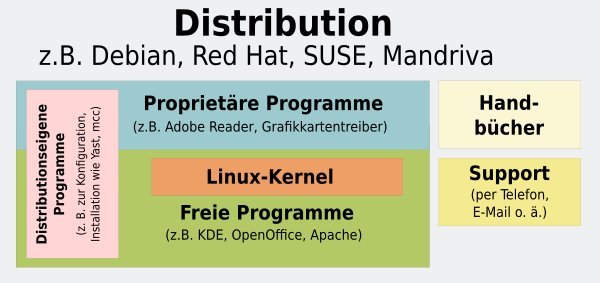
\includegraphics[scale=0.1]{images/distros1.jpg}}
	    \hspace{30px}
	    \fbox{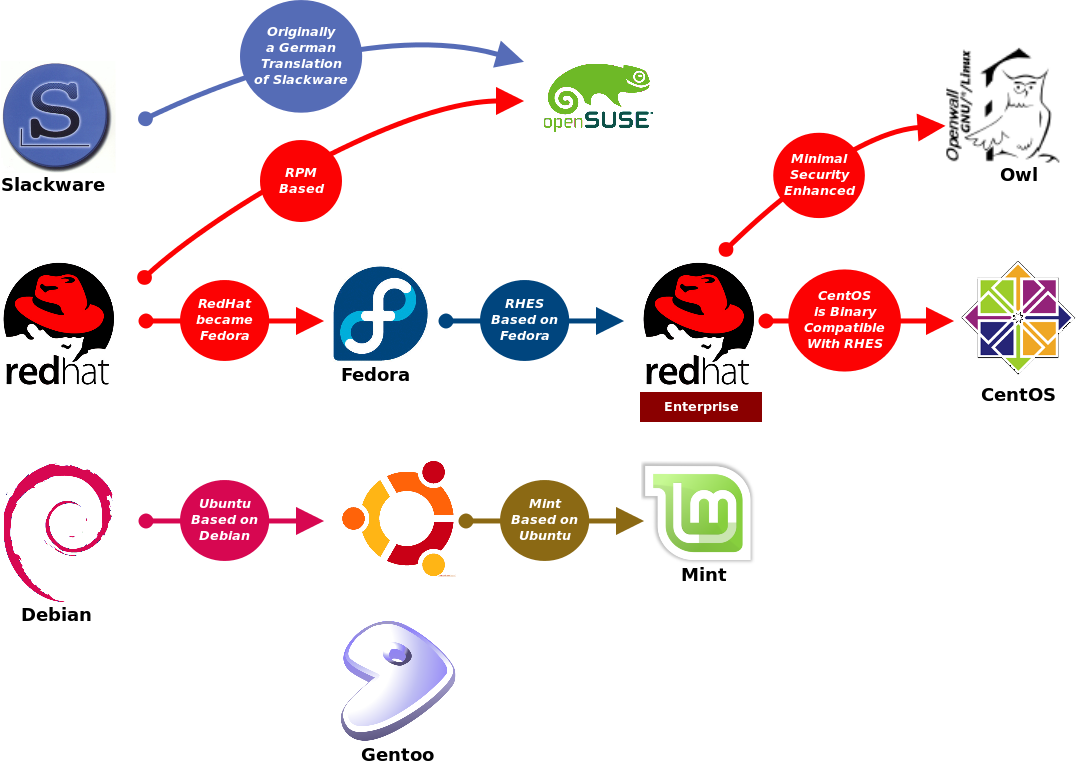
\includegraphics[scale=0.1]{images/distros2.png}}
	    \hspace{30px}
	\end{figure}
\end{frame}

\begin{frame}
	\frametitle{Organización física de discos}
	\begin{figure}
	    \fbox{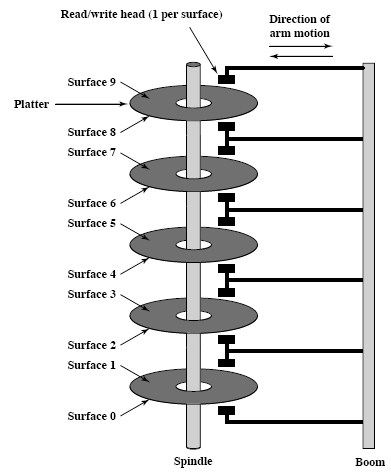
\includegraphics[scale=0.4]{images/hdd1.png}}
	\end{figure}
\end{frame}

\begin{frame}
	\frametitle{Organización física de discos (cont.)}
	\begin{figure}
	    \fbox{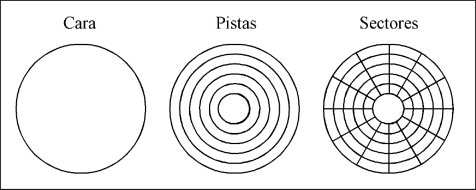
\includegraphics[scale=0.5]{images/hdd2.jpg}}
	\end{figure}
\end{frame}

\begin{frame}
	\frametitle{Organización física de discos (cont.)}
	\begin{figure}
	    \fbox{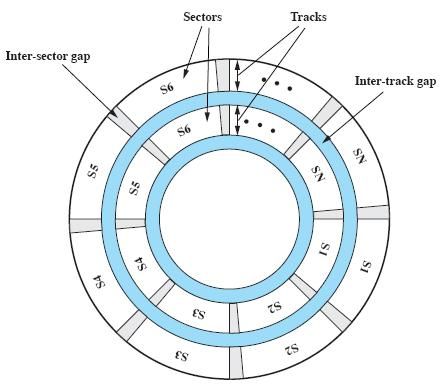
\includegraphics[scale=0.4]{images/hdd3.jpeg}}
	\end{figure}
\end{frame}

\begin{frame}
	\frametitle{Conceptos para la instalación - \textbf{MBR}}
	\begin{itemize}
		\item Sector reservado del disco físico (cilindro 0, cabeza 0, sector 1)
		\item Existe un MBR en todos los discos
		\item Si existiese más de un disco rígido en la máquina, sólo un es designado como \textit{Primary Master Disk}
	\end{itemize}
\end{frame}

\begin{frame}
	\frametitle{Conceptos para la instalación - MBR (cont.)}
	\begin{itemize}
		\item El tamaño del MBR coincide con el tamaño estándar de sector, 512 bytes:
		\begin{itemize}
			\item Los primeros bytes corresponden al \textit{Master Boot Code} (MBC)
			\item A partir del byte 446 está la tabla de particiones. Es de 64 bytes
			\item Al final existen 2 bytes libres o para firmar el MBR
		\end{itemize}
		\item Es creado con algún utilitario	
		\item El MBC es un pequeño código que permite arrancar el SO
		\item La última acción del \textit{BIOS} es leer el MBC. Lo lleva a memoria y lo ejecuta		
		\item Si se tiene un sistema instalado $\rightarrow$ bootloader de MBC típico. Sino $\rightarrow$ uno diferente (\textit{multietapa})		
	\end{itemize}
\end{frame}

\begin{frame}
	\frametitle{Conceptos para la instalación - Particiones}
	\begin{itemize}
		\item Es una forma de dividir lógicamente el disco físico:
		\begin{itemize}
			\item \emph{DOS} y \emph{W95} no pueden manejar filesystems mayores a 2GB
			\item Cada sistema operativo es instalado en una partición separada
			\item Cada partición se formatea con un tipo de filesystem destino (\textit{fat}, \textit{ntfs}, \textit{ext}, etc.)
			\item Es una buena práctica separar los datos del usuario de la aplicaciones y/o sistema operativo instalado
			\item Tener una partición de \emph{restore} de todo es sistema
			\item Poder ubicar el Kernel en una partición de solo lectura, o una que ni siquiera se monta (no está disponible para los usuarios)
			\item Particionar demasiado un disco puede tener desventajas: ¡pensar..!
		\end{itemize}
	\end{itemize}
\end{frame}

\begin{frame}
	\frametitle{Conceptos para la instalación - Particiones (cont.)}
	\begin{itemize}
		\item Debido al tamaño acotado en el MBR para la tabla de particiones:
		\begin{itemize}
			\item Se restringe a 4 la cantidad de particiones primarias
			\item 3 primarias y una extendida con sus respectivas particiones lógicas
		\end{itemize}
		\item Una de las 4 particiones puede ser extendida, la cual se subdivide en volúmenes lógicos
		\item Partición primaria: división cruda del disco (puede haber 4 por disco). Se almacena información de la misma en el MBR
		\item Partición extendida: sirve para contener unidades lógicas en su interior. Solo puede existir una partición de este tipo por disco. No se define un tipo de FS directamente sobre ella
		\item Partición lógica: ocupa la totalidad o parte de la partición extendida y se le define un tipo de FS. Las particiones de este tipo se conectan como una lista enlazada
	\end{itemize}
\end{frame}

\begin{frame}
	\frametitle{Conceptos para la instalación - Particiones (cont.)}
	\begin{itemize}
		\item Como mínimo es necesario una partición (para el /)
		\item Es recomendable crear al menos 2 (/ y \textit{SWAP})
		\item Para crearlas, se utiliza software denominado \textbf{particionador}. Existen 2 tipos:
		\begin{itemize}
			\item Destructivos: permiten crear y eliminar particiones (fdisk)
			\item No destructivo: permiten crear, eliminar y modificar particiones (fips, gparted) $\leftarrow$ generalmente las distribuciones permiten hacerlo desde la interfaz de instalación
		\end{itemize}
		\pause
		\item \textcolor{orange}{¿Para qué podríamos crear otras particiones?}
	\end{itemize}
\end{frame}

\begin{frame}
	\frametitle{Nuestro ambiente de trabajo}
	\begin{itemize}
		\item Vamos a trabajar en un ambiente controlado $\rightarrow$ \emph{VirtualBox}
		\item Necesitamos crear una máquina virtual y asignarle recursos
		\item Booteamos la máquina virtual iniciando desde algún medio de instalación
		\item Seguimos las instrucciones de instalación
		\item Verificamos que podamos arrancar el/los sistemas operativos instalados
	\end{itemize}
\end{frame}

\begin{frame}
	\frametitle{Particionado de discos}
	\begin{itemize}
		\item Particionando - 3 escenatios posibles:
		\begin{itemize}
			\item Usar espacio libre no particionado
			\item Usar partición no usada
			\item Usar espacio libre de una partición actvia (más complicado):
			\begin{itemize}
				\item Cambio destructivo
				\item Cambio no destructivo
			\end{itemize}
		\end{itemize}
		\item En nuestra instalación:
		\begin{itemize}
			\item /dev/hda1: DOS con Wndows (2 GB) $\leftarrow$ ¡es mucho!
			\item /dev/hda2: /boot $\rightarrow$ 60 MB aproximadamente
			\item /dev/hda3: / $\rightarrow$ 6 GB aproximadamente
			\item /dev/hda4: área de intercambio (SWAP)
		\end{itemize}
	\end{itemize}
\end{frame}

\begin{frame}
	\frametitle{Verificando la configuración de nuestro disco}
	\begin{itemize}
		\item Desde Windows: utilizamos el administrador de discos
		\item Desde DOS: usamos fdisk
		\item Para instalar un nuevo SO necesitamos espacio libre sin particionar
		\item Si no lo tenemos, debemos generarlo. Para esto existen diversos escenarios:
		\begin{itemize}
			\item Eliminar una partición existente
			\item Redimensionar una partición
		\end{itemize}
		\item \textcolor{orange}{¿Qué ocurre en cada caso? ¿Qué software vamos a usar?}
	\end{itemize}
\end{frame}

\begin{frame}
	\frametitle{Eumuladores/Virtualizadores}
	\begin{itemize}
		\item Para los fines de este curso, permiten virtualizar plataformas
		\item Permite que en un equipo puedan correr varios SO en forma simultánea compartiendo recursos de hardware
		\item El pionero en esta tecnología fue \emph{IBM} con el IBM System/360 en los años 1960
		\begin{figure}[h]
			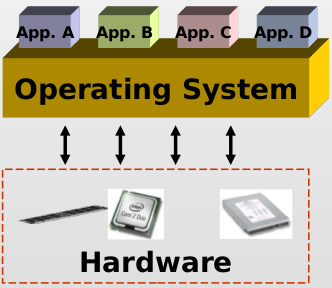
\includegraphics[scale=0.3]{images/virt1.png}
			\hspace{30px}
			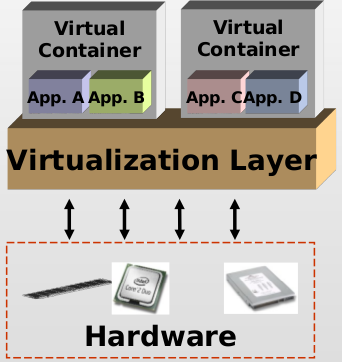
\includegraphics[scale=0.3]{images/virt2.png}
		\end{figure}
	\end{itemize}
\end{frame}

\begin{frame}
	\frametitle{Eumuladores/Virtualizadores (cont.)}
	\begin{itemize}
		\item Básicamente se pueden considerar 3 tipos:	
		\begin{itemize}
			\item Emulación:
			\begin{itemize}
				\item Emulan hardware
				\item Tienen que implementar todas las instrucciones de la CPU
				\item Es muy costosa y poco eficiente
				\item Permite ejecutar arquitecturas diferentes a las soportadas por el hardware
			\end{itemize}
			\item Virtualización completa:
			\begin{itemize}
				\item Permiten ejecutar SO huéspedes en un sistema anfitrión (host)
				\item Utilizan en el medio un hypervisor o monitor de máquinas virtuales
				\item El SO huésped debe estar soportado en la arquitectura anfitriona
				\item Es más eficiente que la emulación (\emph{Intel-VT} y \emph{AMD-V})
			\end{itemize}
			\item Paravirtualización:
			\begin{itemize}
				\item Permite correr SOs modificados exclusivamente para actuar en entornos virtualizados
				\item Mayor eficiencia que la virtualización
			\end{itemize}			
		\end{itemize}		
	\end{itemize}
\end{frame}

\begin{frame}
	\frametitle{Eumuladores/Virtualizadores (cont.)}
	\begin{itemize}
		\item Las principales diferencias entre ellos son:
		\begin{itemize}
			\item Los virtualizadores aprovechan el CPU sobre la que están trabajando, lo cual los hace más veloces
			\item En un emulador se puede correr cualquier arquitectura. En un virtualizador solo se puede correr la arquitectura virtualizada
		\end{itemize}
		\begin{figure}[h]
			
\includegraphics[scale=0.2]{images/bochs.png}
			\hspace{30px}
			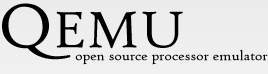
\includegraphics[scale=0.2]{images/quemu.png}
			\hspace{30px}
			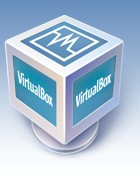
\includegraphics[scale=0.2]{images/virtualbox.png}
			\hspace{30px}
			
\includegraphics[scale=0.2]{images/vmware.png}
			\hspace{30px}
			
\includegraphics[scale=0.2]{images/xen.png}
		\end{figure}		
	\end{itemize}
\end{frame}

\begin{frame}
	\frametitle{Gestor de arranque}
	\begin{itemize}
		\item La finalidad del bootloader es la de cargar una imagen de \textit{Kernel} (sistema operativo) de alguna partición para su ejecución
		\item Se ejecuta luego del código del BIOS		
		\item Existen 2 modos de instalación:
		\begin{itemize}
			\item En el MBR (puede llegar a utilizar \textit{MBR gap})
			\item En el sector de arranque de la particion raíz o activa (\textit{Volume Boot Record})
		\end{itemize}
		\item \emph{GRUB}, \emph{LILO}, \emph{NTLDR}, \emph{GAG}, \emph{YaST}, etc.
	\end{itemize}
\end{frame}

\begin{frame}[fragile]
	\frametitle{Grub Legacy}
	\begin{itemize}
		\item \textbf{GRand} \textbf{Unified} \textbf{Bootloader}: gestor de arranque múltiple más utilizado
		\item En el MBR solo se encuentra la fase 1 del que solo se encarga de cargar la fase 1.5
		\item Fase 1.5: ubicada en los siguientes 30 KB del disco (\textit{MBR gap}). Carga la fase 2
		\item Fase 2: interfaz de usuario y carga el Kernel seleccionado
		\item Se configura a través del archivo \textcolor{orange}{/boot/grub/menu.lst}
		\item Algunas líneas:
		\begin{itemize}
			\item default: define el SO por defecto a bootear
			\item timeout: tiempo de espera para cargar el SO por defecto
		\end{itemize}
		\begin{lstlisting}
title Debian GNU/Linux
root (hd0,1) #(Disco,Particion)
kernel /vmlinuz-2.6.26 ro quiet root=/dev/hda3
initrd /initrd-2.6.26.img
		\end{lstlisting}		
	\end{itemize}
\end{frame}

\begin{frame}
	\frametitle{Grub 2}
	\begin{itemize}
		\item Utilizado en la mayoria de las distribuciones
		\item Dentro de sus mejoras, incluye el soporte a nuevas arquitecturas, soporte de caracteres no ASCII, idiomas, customización de menúes, etc.
		\item En Grub 2 la fase 1.5 ya no existe más
		\item El archivo de configuración ahora es \textcolor{orange}{/boot/grub/grub.cfg} y no debería editarse manualmente $\rightarrow$ update-grub
		\item Más información en: \url{https://help.ubuntu.com/community/Grub2}
	\end{itemize}
\end{frame}

\begin{frame}
	\frametitle{Proceso de arranque}
	\begin{itemize}
		\item Es el proceso de inicio de una máquina y carga del sistema operativo y se denomina \textit{bootstrap}
		\item En las arquitecturas x86, el \textbf{BIOS (Basic I/O System)} es el responsable de iniciar la carga del SO a través del MBC:
		\begin{itemize}
			\item Está grabado en un chip (\emph{ROM}, \emph{NVRAM})
			\item En otras arquitecturas también existe, pero se lo conoce con otro nombre:
			\begin{itemize}
				\item Power on Reset + IPL en \textit{mainframe}
				\item OBP (OpenBoot PROM): en \textit{SPARC}
			\end{itemize}
		\end{itemize}
		\item Carga el programa de booteo (desde el MBR)
		\item El gestor de arranque lanzado desde el MBC carga el Kernel:
		\begin{itemize}
			\item Prueba y hace disponibles los dispositivos
			\item Luego pasa el control al proceso \textbf{init}
		\end{itemize}
		\item El proceso de arranque se ve como una serie de pequeños programas de ejecución encadenada
	\end{itemize}
\end{frame}

\begin{frame}
	\frametitle{Problemas del arranque basado en BIOS}
	\begin{itemize}
		\item Es de la década del 80
		\item La última acción del BIOS es leer el MBC del MBR
		\item El firmware del BIOS no facilita la lectura de filesystems
		\item El MBC no puede ocupar más de 446 bytes
		\begin{itemize}
			\item Por ejemplo Grub, utiliza los 446 bytes del MBR y luego utiliza sectores del disco adyacentes que deberían estar libres (\textit{MBR gap})
		\end{itemize}
	\end{itemize}
\end{frame}

\begin{frame}
	\frametitle{Extensible Firmware Interface}
	\begin{itemize}
		\item EFI: nexo entre el SO y el firmaware
		\item Utiliza el sistema \textbf{GPT} (GUID partition table) para solucionar limitaciones del MBR, como la cantidad de particiones
		\item GPT especifica la ubicación y formato de la tabla de particiones en un disco duro
		\item Es parte de EFI. Puede verse como una sustitución del MBR
		\item La especificación EFI es propiedad de Intel
		\begin{figure}
			\centering
			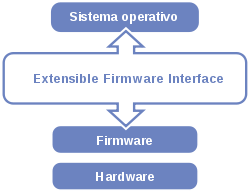
\includegraphics[scale=0.3]{images/efi.png}
		\end{figure}
	\end{itemize}
\end{frame}

\begin{frame}
	\frametitle{GPT}
	\begin{itemize}
		\item Se mantiene un MBR para tener compatibilidad con el esquema BIOS
		\item GPT usa un modo de direccionamiento lógico (logical block addressing \textbf{LBA}) en lugar de \textit{cylinder-header-sector}
		\item El MBR ``heredado'' se almacena en el LBA 0
		\item En el LBA 1 está la cabecera GPT. La tabla de particiones en sí está en los bloques sucesivos
		\item La cabecera GPT y la tabla de particiones están escritas al principio y al final del disco (redundancia)
	\end{itemize}
\end{frame}

\begin{frame}[fragile]
	\frametitle{GPT (cont.)}
	\begin{figure}
		\centering
		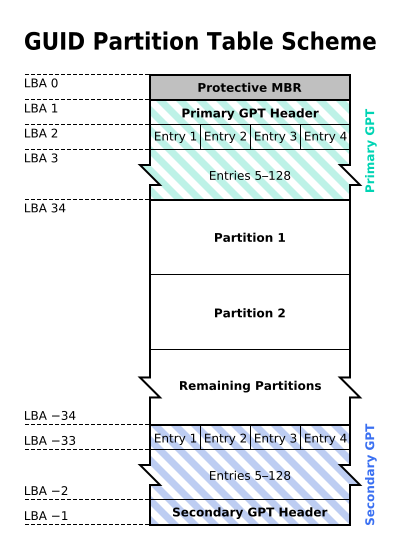
\includegraphics[scale=0.3]{images/gpt.png}
	\end{figure}
\end{frame}

\begin{frame}
	\frametitle{Unified Extensible Firmware Interface}
	\begin{itemize}
		\item UEFI Forum
		\begin{itemize}
			\item Alianza entre varias compañias con el objetivo de modernizar el proceso de arranque
			\item Representantes de AMD, American Megatrends, Apple, HP, Dell, IBM, Insyde Software, Intel, Lenovo, Microsoft, Phoenix Technologies
			\item EFI es propiedad de Intel
			\item UEFI es propiedad del UEFI Forum
			\item UEFI aporta criptografía, autenticación de red y una interface gráfica
		\end{itemize}
	\end{itemize}
\end{frame}

\begin{frame}
	\frametitle{UEFI (cont.)}
	\begin{itemize}
		\item Define la ubicación de gestor de arranque
		\item Define la interfaz entre el gestor de arranque y el firmware
		\item Expone información para los gestores de arranque con:
		\begin{itemize}
			\item Información de hardware y configuración del firmware
			\item Punteros a rutinas que implementan los servicios que el firmware ofrece a los bootloaders u otras aplicaciones UEFI
			\item Provee un \textit{BootManager} para cargar aplicaciones UEFI (e.j.: Grub) y drivers desde un UEFI filesystem
			\item El booloader ahora es un tipo de aplicación UEFI:
			\begin{itemize}
				\item El Grub será una aplicación UEFI, que reside en el UEFI filesystem donde están los drivers necesarios para arrancar el sistema operativo (FAT32)
				\item Para el Grub deja de ser necesario el arranque en varias etapas.
			\end{itemize}
		\end{itemize}
	\end{itemize}
\end{frame}

\begin{frame}
	\frametitle{Secure Boot}
	\begin{itemize}
		\item Propone mecanismos para un arranque libre de código malicioso
		\item Las aplicaciones y drivers UEFI (imágenes UEFI) son validadas para verificar que no fueron alteradas
		\item Se utilizan pares de claves asimétricas
		\item Se almacenan en el firmware una serie de claves publicas que sirven para validar que las imágenes estén firmadas por un proveedor autorizado
		\item Si la clave privada está vencida o fue revocada la verificación puede fallar
	\end{itemize}
\end{frame}
